\chapter{Background}

\section{Natural language Processing}
  Natural language processing (\GLS{NLP}) consists of a set of methods that operate on natural language (language that naturally evolved among humans) to solve tasks like translation, question answering, text summarization, and interaction with spoken language.
  While humans can intuitively solve these tasks, machines require a whole batch of preprocessing steps to utilize such raw data and cope with the redundancy in language and facilitate the otherwise not accessible underlying rules (including but not limited to grammar).
  Fig. \ref{fig:pipeline} shows a pipeline that illustrates the language wrangling steps common in NLP for information extraction.

\begin{figure}[h!]
  \centering
  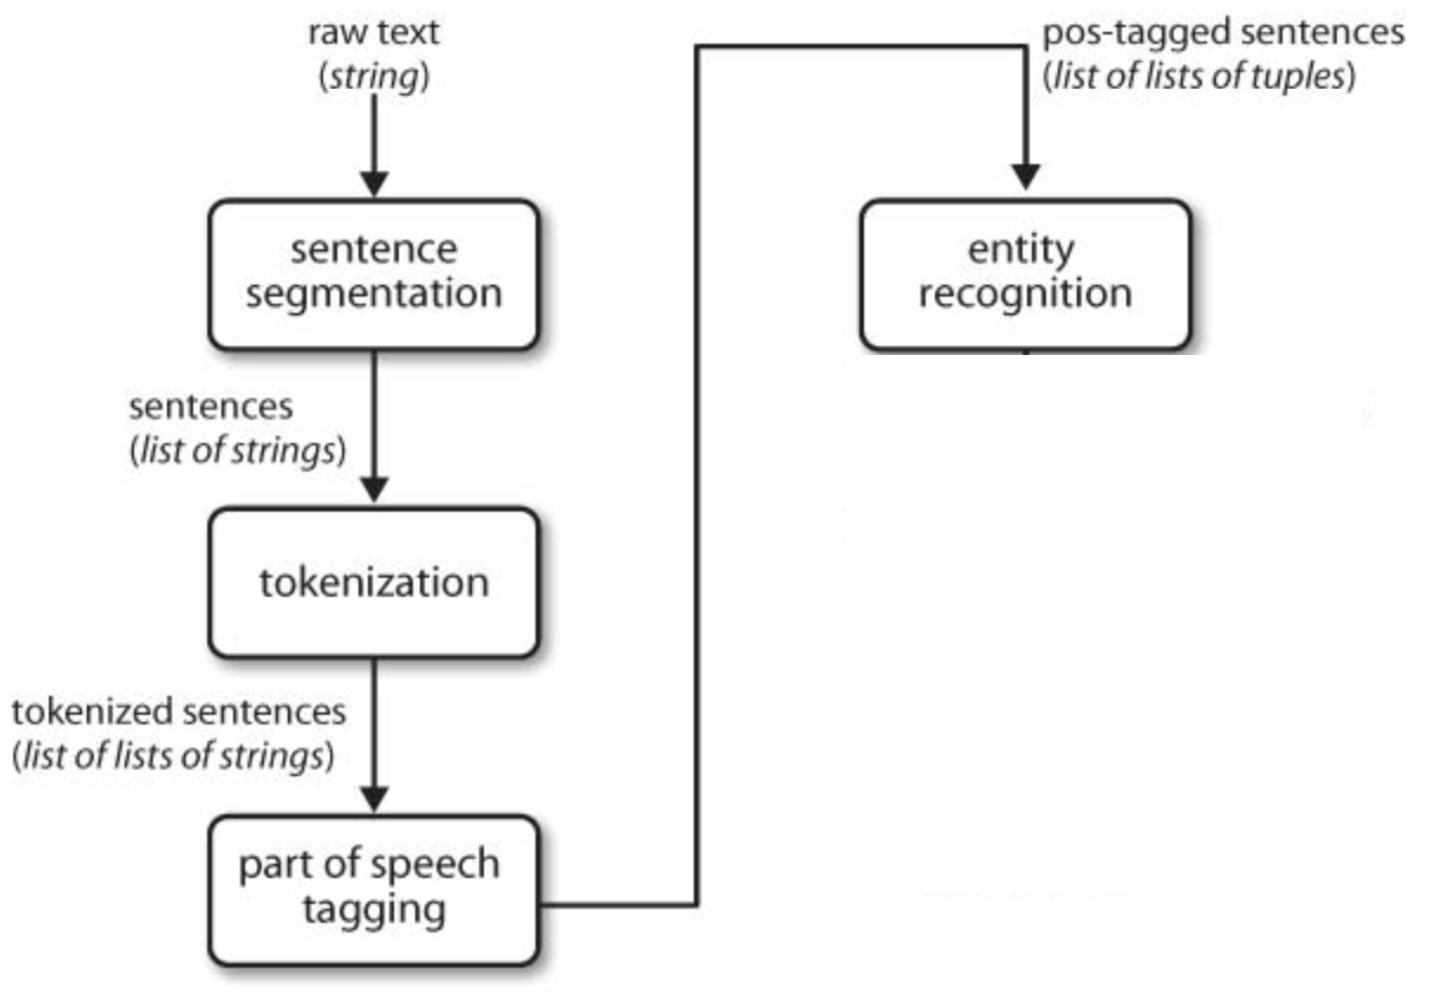
\includegraphics[scale=0.4]{pipeline.png}
  \caption{An illustration of a typical pipeline for information extraction in NLP. The pipeline starts with the raw text and undergoes several preprocessing steps (indicated by a rectangle) yielding intermediate output (placed next to the arrows). The final output can be a list of tuples of the entity and the corresponding word like \texttt{[(ORG, \textquotesingle Bayer\textquotesingle), (LOC, \textquotesingle Baveria\textquotesingle)]} (adapted from \cite{Bird2009}).}
\label{fig:pipeline}
\end{figure}

\subsection{Stop Words}
  Assuming we want to analyze texts on word level, we might be looking for
  words that appear more often than others or only appear in certain texts.
  This information can tell us a lot about the topic or sentiment of a text.
  Suppose we find that a text is frequently mentioning \textit{Brexit} more than any other text.
  Then we can deduct that this text might be a (news) article and that it is about the exit of Great Britain from the European Union.
  However, we quickly realize that certain words also appear more frequently than others, without revealing much about the content of the text.
  Words like \textit{the, of, than} appear numerously in every English text independently of the topic or the source.
  Such words first received particular attention when \cite{Luhn1960} identified their property to obscure target words for further analyzes.
  These words are called \textbf{stop words}\index{stop words}, and there are by now many curated lists of stop words for different languages and tasks \citep{RANKS2019}.

  % In case we want to find, as an example, adjectives and adverbs in a text for a sentiment  them since stop words contain information about the grammatical structure of the text.
  For any NLP algorithm that requires information about the grammatical structure of a text, we want to keep stop words since they convey a substantial part of grammatical information.
  However, should we be interested in the topic or source of the text, then it might be sufficient to search for this information within only a handful of words.
  % Stop words would only distract the machine learning algorithm from words that do convey information about the topic of the text.
  Therefore, it is common practice to remove stop words to improve the performance of classification algorithms \citep{McCallum1998, Lodhi2002, Tong2001}.
  In state-of-the-art neural classifier like described by \cite{Howard2018}, it is not always necessary.

\[\dots\]
% \subsection{Regular Expressions}
%   Regular expressions (\gls{regex}) is an expression using ASCII characters to define a set of strings that this expression matches.
%   Regex consists of meta and literal characters.
%   For a literal character holds that it matches this exact character in some target text.
%   A metacharacter is interpreted and facilitates regexs \citep{Kleene1951}.
%   While these metacharacters vary between different regex libraries, most of them are identical.
%   A literal character combined with a \texttt{*} is a ubiquitous functionality (known as the Kleene star) and means that the literal character may appear $0$ to $n$ times in succession to allow a match.
%   To still be able to use those metacharacters as literal characters, they can be escaped (generally with a backslash).
%   Tokenization (\ref{tokenization}) or stemming (\ref{stemming}) are preprocessing steps in NLP that sometimes use rules formulated as regexs.

\subsection{Tokenization}\label{tokenization}
  A token is an abstraction of a piece of information.
  In NLP this can be a single character, word, punctuation, or sentence.
  The goal in \textbf{tokenization}\index{tokenization} is to split a text into meaningful chunks that obey the rules of the natural language.
  Word tokenization is the cornerstone for the vast majority of NLP pipelines \citep{Webster1992}.
  % Nevertheless, tokens are not equal to what we perceive as an atomic unit in language, and we need to keep in mind that in the case of computers it is just a representation of some (hopefully) UTF-8 code.

  Tokens, however, do not always match how we think about words or sentences which can be shown by the following example.
  If we would formulate simple rules for tokenization, then a definition for a word would be a string enclosed by single white space characters.
  A simple regex for this rule would be \texttt{[a-zA-Z]+} that matches 1 to $n$ (indicated by \texttt{+}) lower or uppercase letter (indicated by \texttt{[a-zA-Z]}) in succession.
  Words delimited by periods would then be a sentence.
  These regexs, however, do not always work as expected.
  The \textit{United States of America} is such an example where our rules would fail.
  They lead to splitting this string into four tokens \mbox{\{\textquotesingle \textit{United}\textquotesingle, \textquotesingle \textit{States}\textquotesingle, \textquotesingle \textit{of}\textquotesingle, \textquotesingle \textit{America}\textquotesingle\}} although these tokens are not independent of each other and thus should be one token.
  Longer names like this one often have acronyms such as the \textit{U.S.A}.
  Following our simple rules, the word \textit{U.S.A} would be split into six tokens \mbox{\{\textquotesingle \textit{U}\textquotesingle, \textquotesingle \textbf{.}\textquotesingle, \textquotesingle \textit{S}\textquotesingle, \textquotesingle \textbf{.}\textquotesingle, \textquotesingle \textit{A}\textquotesingle, \textquotesingle \textbf{.}\textquotesingle\}} since it is mistaken by a sentence.

  On the other hand, using an established tokenizer is also wondering e.g, \textit{don't} is split into \{\textquotesingle \textit{do}\textquotesingle, \textquotesingle \textit{n't}\textquotesingle\} but we know it should be \{\textquotesingle \textit{do}\textquotesingle, \textquotesingle \textit{not}\textquotesingle\} assuming tokens are a representation of words.
  However, since tokens are not meant to be a precise image of natural language words but rather a method to yield word level understanding then \textit{not} represented as \textit{n't} will not worsen any text analysis, if the usage of \textit{n't} is consistent.
  So without a doubt, the \textit{United States of America} or the acronym \textit{U.S.A.} needs to be treated as a single unit for sufficient word-level understanding.
  It is common to use a curated list of expected abbreviations, names, and phrases to avoid bad tokenization.
  To improve sentence tokenization further, one could train an unsupervised sentence boundary detector as described in \cite{Kiss2006}.
  This method extracts the most occurring sentence breaks and learns to discard those that do not to seem to be a valid new sentence.
  The acronym \textit{U.S.A.} will occur only as a fraction compared to more frequent sentence breaks.
  The most common one will be lower-case letters followed by a whitespace, a period, and then an upper-case letter in standard literature or new lines in online chats.

  Sentence tokenization is based on word-tokenization and is also part of most text analyzes.
  It becomes essential, for example, if a text includes logical elements (like paragraphs or chapters) that need to be handled differently as in news summarization where the core content is more likely to be found in the first paragraph.

\subsection{POS-Tagging}
  Although tasks like text classification perform already well with a text that only has been tokenized, mostly we require further processing to do more language-aware tasks.
  If the grammatical correction of texts is the goal of some NLP pipeline, then it goes without saying that we need more information about the grammatical function of the extracted token.

  % As an example, we assume a sentence like \textit{``I read a book about grammar that were very helpful"}.
  % A lookup in an English dictionary will yield that every word in this sentence is written correctly, but we know that the sentence is still wrong.
  % We know that \textit{that} refers to \textit{book} and that \textit{book} is singular and hence \textit{that} aswell.
  % But \textit{that} is followed by a plural auxiliary verb (in this case \textit{were}) which makes this sentence wrong.
  % A hypothetical grammar dictionary lookup is not able to detect \textit{that} should be followed by \textit{was} since \textit{that} is written the same when referring to single and plural nouns.
  % To solve this programmatically, we need to find the grammatical number of the noun before the first mentioning of \textit{that} to determine if the grammatical count of the auxiliary verb after \textit{that} is correct.
  We could, for example, want to identify all nouns from a text. This will be an easy task for many words like \textit{car} or \textit{mother}. They can be looked up in an English dictionary which will confirm that these words are nouns. However, words like \textit{meeting} can take different parts of speech (verb or noun).

  To find the noun, we apply \textbf{position-of-speech tagging} (\gls{POS-tagging}).
  A POS-tagger is typically a machine learning model like a decision tree \citep{Marquez98} trained on an annotated corpus like Penn Treebank \citep{PennTreebank}, that already has the right grammatical entities assigned to each word in unstructured texts.
  When the correct grammatical function of all tokens is determined, it is simple to detect the grammatical number of the noun occurring before \textit{that} and hence correct the sentence grammatically.

\subsection{Lemmatization and Stemming}\label{stemming}
  Having a well-tokenized text, we can do descriptive statistics on the text, e.g., by counting the occurrences of tokens or detect tokens that only occur once, so-called \textbf{hapax legomenon}.
  The simplest way to sensibly reason about a text would be to find the most frequent words, given that we removed stop words to infer the subject of a text.
  If the goal were to infer the type of sport based on the most occurring words in sports news we would hope to find a high term frequency for something like \textit{throw} for baseball or \textit{strike} for soccer.
  Merely counting tokens to display the most occurring ones in a text will not be sufficient.
  The words in the text will be used in many forms due to grammatical conjugation.
  For example, \textit{thrown} and \textit{throw} will be treated as unequal tokens by the computer although they mean the same.
  Therefore, we need to transform all words to their infinitive form.

  There are two options: \textbf{stemming}\index{stemming} and \textbf{lemmatization}\index{lemmatization}.
  Stemming only prunes the end of words following rules.
  These rules are specified as regular expressions which try to exploit regularities in language to infer the infinitive form.
  However, they will not always reliably work due to special cases and ambiguities of natural language.
  One common rule among stemmers is the removal of \textit{ing} at the end of a lower case word to transform a word into its infinitive form.
  This rule works correctly in most cases but fails for words like \textit{lying} that the stemmer transforms to \textit{ly} which is a not desired behavior.

  Lemmatization is a more sophisticated method.
  First, it uses a grammatical database lookup instead of rules and therefore will be able to transform \textit{lying} correctly to \textit{lie}.
  Second, it incorporates POS-tagging to determine how words need to be transformed based on their grammatical function \citep{Muller2015}.
  If the word \textit{meeting} is used as a noun, we do not want to transform it to \textit{meet} but keep it like it is.
  Lemmatization produces better results than stemming \citep{Balakrishnan2014} for a higher cost of computation.


\subsection{(Disease) Named-Entity Recognition}
  Named-entity recognition (\GLS{NER}) is a step placed towards the end of an NLP pipeline (Fig. \ref{fig:pipeline}).
  After sentences and words have been tokenized, and POS-tagging was applied, it might be important for some learning algorithms to know the named-entity of words.
  Typical examples are the recognition of names of persons or companies, and numerical entities, like time, dates, and money \citep{Nadeau2009}.
  This recognition might be part of some NLP pipeline, but it also can be part of a pipeline for information retrieval (\GLS{IR}).
  The goal of IR is the extraction of specific information and their subsequent storage in a database to structure a large amount of data that is difficult to access \citep{Manning2008, Wei2011}.

  The reason NER is not covered merely by a dictionary lookup but a separate module in a pipeline is the difficulty to deal with ambiguous words like \textit{Apple}.
  When the word \textit{Apple} is at the beginning of a text, it is unclear whether it stands for the fruit or a tech company.
  While in the beginning, NER consisted of handcrafted rules and heuristics \citep{Rau1991}, NER is now a classification problem that can be solved through supervised learning, capable of learning named entities with hidden Markov models, decision trees, or conditional random fields \citep{Nadeau2009}.
  Though, there is a shift towards un/semi-supervised methods that infer features (as neural networks) and outperform feature-engineered systems (as decision trees) \citep{Yadav2018}.

  In the medical field, such ambiguities rise not because the proper names are so indistinguishable from other common words, but because there are many forms how to write a disease name and equally many abbreviations (e.g., \textit{cancer}, \textit{carcinoma}, \textit{malignant tumor}, \textit{CA}).
  To reason from medical texts, it is necessary to identify those utterances that are most likely representing a disease.
  Thus, disease-NER is a crucial processing step in this domain.
  However, benchmarks also showed that in highly standardized, text dictionary lookups perform equally well \citep{Jimeno2007}.
  Therefore, the exact procedure to perform disease NER depends on the source of interest.

\subsection{Corpus}
  A \textbf{corpus}\index{corpus} is an organized collection of (related) text documents that are simple to access. They can be annotated (as required for training POS-tagger) or preprocessed (e.g., tokenized) \citep{Bengfort2018}.
  Preprocessing, however, can be time-intensive especially for large amounts of data and this process irreversibly changes the raw text.
  Thus, each intermediate step should be stored in the corpus as well.
  This way, quality control is assured, replacement of preprocessing steps is streamlined, and repeated computations or even human labor is avoided.
  Optimally, a corpus is easily accessible and safely stored since it contains laboriously created data.
  NoSQL databases are advantageous for corpus saving due to their minimal overhead and allow access to data that would be too large for a normal machine.
  This way corpora can easily be shared by providing access to the database.
  Alternatively, they can be stored as a folder system containing \texttt{.txt}, \texttt{.XML}, or \texttt{.JSON} files.

\section{Machine Learning}
  Machine learning (\GLS{ML}) is an attempt to make the computer learn. \citeauthor{Mitchell1997} described learning broadly as,
  %
  \begin{quote}
    ``A computer program is said to \textbf{learn} from experience $\mathcal{E}$ with respect to some class of task $\mathcal{T}$ and performance measure $\mathcal{P}$, if its performance at tasks in $\mathcal{T}$, as measured by $\mathcal{P}$, improves with experience $\mathcal{E}$.''
  \end{quote}
  %
  There are, however, ML algorithms that not necessarily define $\mathcal{E}$.
  Making experience from seeing labeled examples is called \textbf{supervised learning}\index{supervised learning} and learning a model without labels is called \textbf{unsupervised learning}\index{unsupervised learning}.
  % Therefore, one could also consider the following definition  \[f: X \rightarrow \hat{y}\] where $f$ is a machine learning model that takes some data $X$ and tries to predict the most likely label $\hat{y}$ where $\hat{y} \approx y$ and $y$ being the true label.

\subsection{Bag-Of-Words}\label{section:bow}
  It is typical in a machine learning task that large amounts of data can make explicit feature engineering unnecessary.
  Also, instead of requiring too much domain knowledge, it is preferred to let the algorithm determine important features.
  One typical example of this in NLP is the \textbf{bag-of-words}\index{bag-of-words} approach.

  It is particularly challenging to model language because of its entangled grammar, all its special cases, idioms, and ambiguity.
  Therefore, we can try to analyze a text based only on the occurrences of the words in the text without their grammatical context.
  We do so by tokenizing a text, lemmatize the tokens and operate on the set of words left after this preprocessing as our set of features.

  A typical example of this simple approach is spam detection.
  Given a set of emails and labels \textsl{spam} and \textsl{not spam}, a machine learning model could learn to classify \textsl{spam}.

\subsection{Imbalanced Class Problem}
  When it is required to detect seldom events, like cancer in patients through imaging, the performance of the classifier suffers from \textbf{imbalanced classes}\index{imbalanced classes}.
  In the cancer example, this would mean that images showing a tumor are much rarer than those without cancer.
  A classifier then tends to classify most input as the majority class, i.e., the patient not having cancer, which would yield a high accuracy but is fatal for the patient.
  The accuracy (the relative amount of correctly classified classes) in this case is not a useful measure, but there are many ways to tackle the class imbalance problem.

  One way is cost-sensitive learning, which treats different misclassifications differently as opposed to cost-insensitive learning that only tries to maximize accuracy.
  Thus, in cost-sensitive learning, it is possible to explicitly model the, e.g., minimization of false negatives such as in the cancer detection example by introducing a cost function for misclassifications or shift the decision threshold of the classifier towards the imbalanced classes \citep{Ling2008}.

  Another way is using up- and downsampling methods.
  A naive downsampling approach would be to discard data of the majority class until the classes are balanced.
  The naive counterpart to downsampling is the duplication of minority class instances and is called upsampling.
  However, there are more sophisticated methods, that will downsample redundant majority class instances or synthesize data, in order to create novel examples of the minority class.
  One well performing upsampling method is called \textbf{Adaptive Synthetic Sampling Approach for Imbalanced Learning} (\GLS{ADASYN}) \citep{He2008}.
  The general procedure of ADASYN is described as,
  \begin{align}
    d &= \frac{m_s}{m_l} \\
    G &= (m_l - m_s) \cdot \beta \\
    r_i &= \frac{\Delta_i}{K}, i=1, \dots, m_s \\
    \hat{r} &= \frac{r_i}{\sum_{i=1}^{m_s} r_i } \\
    g_i &= \hat{r} \cdot G \\
    \forall \boldsymbol{x_i} \text{ repeat } g_i \text{ times: } \boldsymbol{s_i} &= \boldsymbol{x_i} + (\boldsymbol{x_{zi}} - \boldsymbol{x_i}) \cdot \lambda
  \end{align}
  where $d$ is the degree of imbalance of the small and large class ($m_s$ and $m_l$ respectively), $G$ is the number of synthetic data examples required to achieve a class balance of $\beta \in [0,1]$.
  $\Delta_i$ is the number of examples having $K$ nearest neighbors of $\boldsymbol{x_i}$ from the majority class, (2.4) is a normalization step, and $g_i$ is the number of synthetic data instances that need to be generated for each minority example $\boldsymbol{x_i}$.
  (2.6) is the main algorithm where for each data point $\boldsymbol{x_i}$, $g_i$ synthesizations are conducted.
  Thereby, $\boldsymbol{x_{zi}}$ is a random data example from the $K$ nearest neighbors, and $\lambda \in [0,1]$ is a random number.

  Finally, a good performance measure is required to evaluate the classifier's learning progress.
  Accuracy, as illustrated before, is not a reliable indicator in an imbalanced two class dataset.
  The \textbf{Index of Balanced Accuracy} (\GLS{IBA}), however, tries to take the imbalance into account and is defined as, \[IBA_{\alpha} = (1 + \alpha \cdot (TPrate - TNrate)) \cdot TPrate \cdot TNrate \] where 0 $\leq \alpha \leq 1$ and $\alpha$ being a dominance index, that needs to be fine-tuned based on how significant the dominating class is supposed to be.

\subsection{Naive Bayes Classifier}\label{section:nbc}
  The \textbf{naive Bayes classifier}\index{naive Bayes classifier} (\GLS{NBC}) is a probabilistic classifier.
  It describes a set of algorithms capable of learning to infer a class given a set of features and labels.
  The NBC is defined as,
  \begin{align}
    \boldsymbol{x} &= \{x_1, x_2, \dots, x_n\} \\
    \mathcal{C} &= \{\mathcal{C}_k \: | \: k \in K \} \\
    p(\mathcal{C}_k|\boldsymbol{x}) &= \frac{p(\boldsymbol{x} |\mathcal{C}_k) p(\mathcal{C}_k)} {p(\boldsymbol{x})} \\
    p(\mathcal{C}_k|\boldsymbol{x}) &= \frac{p(x_1 |\mathcal{C}_k)
                                         p(x_2 |\mathcal{C}_k) \dots
                                         p(x_n |\mathcal{C}_k)
                                         p(\mathcal{C}_k)}{p(\boldsymbol{x})}
  \end{align}
  where $\boldsymbol{x}$ is a data point which consists of $n$ features.
  $\mathcal{C}$ is the set of all classes, and $p(\mathcal{C}_k|\boldsymbol{x})$ is the probability $\boldsymbol{x}$ belonging to class $\mathcal{C}_k$.
  We are allowed to write (2.9) as (2.10) due the independene assumption of the features of $\boldsymbol{x}$,
   \[p(x_i| \{\forall x_j \in \boldsymbol{x} : j \neq i \}, \mathcal{C}_k) \overset{\, \,\,\,x_i\perp\!\!\!\perp \forall x_j}{=} p(x_i|\mathcal{C}_k)\]
  A standard procedure to predict the most likely class that $\boldsymbol{x}$ belongs to, is to find the maximum a posteriori probability
  \begin{gather}
    \argmax_{k \in \mathcal{C}} p(\mathcal{C}_k|\boldsymbol{x})
  \end{gather}
  To evaluate (2.10), we need to take the product of the probabilities of the features given the class and then consider the class with the highest probability for the classification as in (2.11).

  Note, the classifier is named \emph{naive} because we assume that every feature in the vector $\boldsymbol{x}$ is independent, i.e., there is no correlation between them.
  This assumption is most of the time wrong, but in practice, NBC still performs very well \citep{Rish2001}.


\subsubsection{Multinomial Naive Bayes for Text Classification}
  For classifying texts based on the words they contain as in the bag-of-words approach, we can apply multinomial naive Bayes as follows,
  \begin{align}
    \mathcal{C} &= \{\mathcal{C}_k \: | \: k \in K \} \\
    \boldsymbol{t} &= \{c_1, c_2, \dots, c_n\} \\
    \boldsymbol{T}_{k} &= \{\boldsymbol{t}_d | \forall d \in \mathcal{D}_{\mathcal{C}_{k}}\} \\
    p({t_{k,i}}|\mathcal{C}_k) &= \frac{t_{k, i}}{\sum_{\forall t_j \in \boldsymbol{T}_k} t_{k, j}} \\
    p(\mathcal{C}_k|\boldsymbol{t}_d) &\propto p(\mathcal{C}_k) \prod_{i=1}^{|\boldsymbol{t}_d|}  p(t_{d,i}|\mathcal{C}_k)
  \end{align}
  Where $\mathcal{C}$ is the set of text classes, and $\boldsymbol{t}$ contains the token counts of the whole vocabulary, $c_i$ being the occurrence count of term $i$.
  $\boldsymbol{T}_k$ is a matrix where the token counts $c$ are the columns, and the documents $d$ the rows consisting of all documents $\mathcal{D}$ from class $\mathcal{C}_k$.
  To calculate the likelihood of $p({t_{k,i}}|\mathcal{C}_k)$ we divide the occurrence of token $t_{k,i}$ by the sum of all token occurrences in the same class $\mathcal{C}_k$.
  Following the independency assumption as in (2.10) we now can calculate $P(\mathcal{C}_k | \boldsymbol{t}_d)$ as the product of the prior $P(\mathcal{C}_k)$ -- the probability of class $\mathcal{C}_k$
  as learned from the training set -- and the probabilities of all the terms $t_{1 \dots n}$ given the prior class.
  For classification, the $\argmax$ as in (2.11) is taken.

  Three problems can occur in text classification that need to be handled.
  First, the high probability of numerical underflow due to the large product of several values $<1$, second, some token $t_i \in \boldsymbol{t_d}$ having a count of $0$ that would nullify the whole product, and third, large disparities of token counts that bias the classification.
  The solution to the underflow problem is to transform (2.16) into log-space which equals to:
  %
  \[log(P(\mathcal{C}_k|\boldsymbol{t}_d)) \propto \log(P(\mathcal{C}_k)) + \sum_{i=1}^{|t_{d}|} \log({p(t_{d,i}|\mathcal{C}_k)}) \]
  %
  To avoid $p({t_{i}}|\mathcal{C}_k)$ becoming $0$ we apply Laplace smoothing\index{Laplace smoothing} to (2.15) which yields
  \[ p({t_{k,i}}|\mathcal{C}_k) = \frac{t_{k, i} + 1}{\sum_{\forall t_j \in \boldsymbol{T}_k} t_{k, j} + 1} \]
  and to avoid a bias towards some exceptionally frequent words, \textbf{term frequency-inverse document frequency}(\gls{tf-idf})\index{tf-idf} corrects this discrepancy by weighting the term frequency as follows,
  \begin{align}
    \operatorname{tf}(t,d) &= \frac{f_{t,d}}{\sum_{t' \in d} f_{t',d}}\\
    \operatorname{idf}(t,d, \mathcal{D}) &= log\left( \frac{|\mathcal{D}|}{|d \in \mathcal{D}: t \in d|}\right)\\
    \operatorname{tf-idf}(t,d, \mathcal{D}) &= \operatorname{tf}(t,d) \cdot \operatorname{idf}(t, d, \mathcal{D})
  \end{align}
  where $f_{t,d}$ is the term frequency of term $t$ in document $d$ and $t'$ is any term in $d$.
  $|\mathcal{D}|$ is the number of documents in the corpus and $|d \in \mathcal{D}: t \in d|$ is the number of documents containing term $t$.
  (2.19) is the final formula that balances discrepancies between term frequencies over several documents.

\subsubsection{Bernoulli Naive Bayes}
  Especially for shorter texts and binary decision (\textsl{spam}, \textsl{not spam}), there is only a small gain to use token counts.
  The Bernoulli variant of the NBC explicitly models the absence and presence of words which is done by a different approach to estimating $p(t_{i}|\mathcal{C}_b)$ (comparison to 2.15).
  The probability of token $t_i$ given some binary class is calculated like,
  \[p(t_{i}|\mathcal{C}_b) = p(t_{i})(1-p(t_{i}))^{(1-b)}\]
  where $b \in \{0,1\}$ and $\mathcal{C}_b$ is the corresponding class.

\subsubsection{Complement Naive Bayes}
  There are cases where the \emph{naive} assumption is particularly ill made. In an unbalanced class problem, the data is skewed towards the larger class which the following table illustrates,

  \begin{table}[h!]
    \centering
    \caption{A statistical evaluation of a coin flip experiment with an imbalanced class. $\theta$ is the probability of a class to yield head (H). We flip one coin in Class 1 and two coins in Class 2 per row. $\operatorname{p}(data)$ is the probability for the seen coin flip. The column Label for H contains the class assignment after the coin flip (adapted from \cite{Rennie2003}).}
    \setlength{\tabcolsep}{1.5em}
    \begin{tabular}{@{}cccc@{}}
      \toprule
      \textbf{Class 1} & \textbf{Class 2} & $\mathbf{p(data)}$ & \textbf{Label for H} \\
      $\theta = 0.25$ & $\theta=0.2$ & & \\
      \midrule
      T & TT & $0.48$ & $none$ \\
      T & \{HT, TH\} & $0.24$ & $Class 2$ \\
      T & HH & $0.03$ & $Class 2$ \\
      H & TT & $0.16$ & $Class 1$ \\
      H & \{HT, TH\} & $0.08$ & $Class 1$ \\
      H & HH & $0.01$ & $none$ \\
      \bottomrule
    \end{tabular}
    \label{table:coinflip}
  \end{table}
  The experiment shown in Tab. \ref{table:coinflip} , that considers each possible outcome of coin flips, suggests a 24\% probability for Class 1 to yield H and 27\% for Class 2, although the probability for Class 1 to yield H is actually higher.
  The proposed solution by \cite{Rennie2003} is to minimize the probability of a vector of word counts \textbf{not} belonging to a class to tackle class imbalance,
  \[\argmin p(\neg\, \mathcal{C}_k) \prod_{i=1}^{|t_{d}|} \frac{1}{p(t_{d,i}|\neg\, \mathcal{C}_k)} \]

\subsection{Support Vector Machine}
  A prominent application of vector space based machine learning is the \textbf{support vector machine} (\GLS{SVM})\index{support vector machine}.
  It is a classification algorithm that is trained in a supervised fashion. It is often used for document classification and performs well even on small data \citep{Manning2008}.
  During training time, the SVM tries to find a decision boundary in the vector space of the training data to separate two classes with a maximal margin.
  This is accomplished by choosing a hyperplane that has a maximum distance to the closest data points of both classes respectively. The margin is defined by those points which are called support vectors (Fig. \ref{fig:svm}).
  %
  \begin{figure}[h]
      \centering
      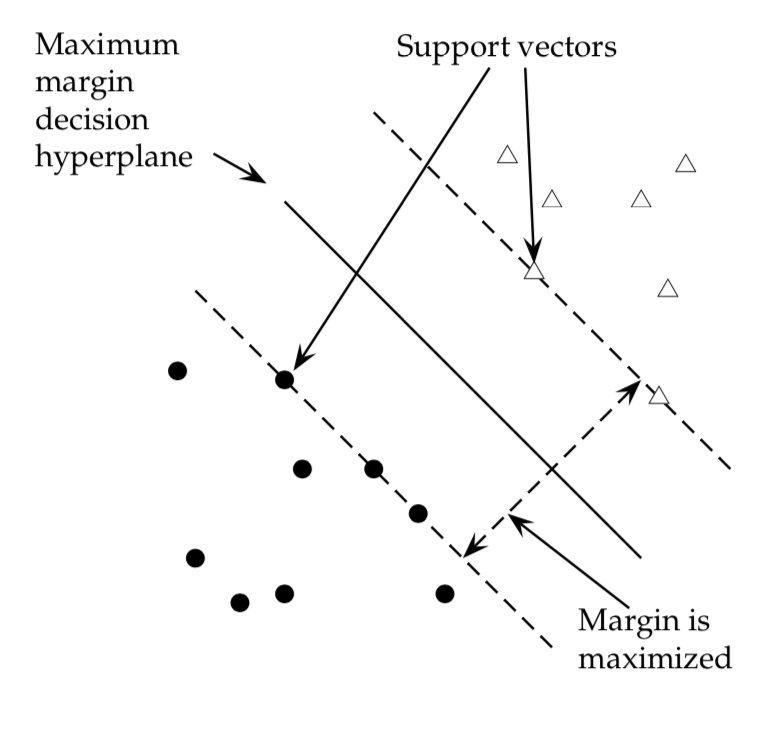
\includegraphics[scale=0.6]{svm.png}
      \caption{An illustration of how support vector machines realize classifications. Black dots and white triangles represent two classes of data points (adapted from \cite{Manning2008}).}
      \label{fig:svm}
  \end{figure}
  %
  For classification, we calculate $\operatorname{f}(\mathbf{x}) = \operatorname{sign}(\mathbf{w}^{T}\mathbf{x} + b)$ where $\mathbf{w}$ is a weight vector orthogonal to the decision hyperplane, $\mathbf{x}$ is the input data point, and $b$ an intercept.
  % Since we try to maximize the margin of the decision hyperplane we are minimizing
  % \frac{1}{2} \mathbf{w^T} \mathbf{w}. Furthermore, we define that the margin has a size of at least 1
  % \[ \forall (\mathbf{x}_i, y_i): y_i(\mathbf{w}^T \mathbf{x} + b) \geq 1 \]
  Training an SVM is an optimization problem which can be solved with, e.g., the Lagrange multiplier, denoted as $\alpha_i$.
  Then,
    \[\mathbf{w} = \sum \alpha_i y_i \mathbf{x}_i \]
    \[b = y_k (1-\zeta_k) - \mathbf{w}^T \mathbf{x}_k \text{ where }k = \argmax_k \alpha_k \]
  where $y_k$ is the label of data point $\mathbf{x}_k$ and all $\alpha_i \neq 0$ are the support vectors. For all $\alpha$ it hols that $0 \leq \alpha \leq C$, where C is a regularization term to control overfit. $\zeta$ is a slack variable that allows the classification with a soft margin, i.e., drawing a margin that classifies some training data points incorrectly for a penalty equals to $\zeta$.
  The classification function then is $\operatorname{f}(\mathbf{x}) = \operatorname{sign}(\sum \alpha_i y_i \mathbf{x}^{T}_i\mathbf{x} + b)$.
  % we try to minimize $\frac{1}{2} |\mathbf{w}|$ and try to satisfiy $\forall {(\mathbf{x}_i,y_i)}: y_i(\mathbf{w}^{T}_{i} \mathbf{x}_i + b ) \geq 1$. This is an optimization problem that can be solved with the Lagrange multiplier.
  There, however, exists much faster, more scalable solutions for training SVMs that I will not thematize.

  % Two classes might be linearly separable, but often noisy data will increase the difficulty to find the correct decision boundary.
  % A solution to this is to define a \emph{slack variable} $\zeta$ which allows some data point $\mathbf{x}_i$ to not meet the margin requirement at a cost equal to the value of $\zeta_i$.
  % We then rewrite the optimization problem as follows,
  % \[ \frac{1}{2} \mathbf{w^T} \mathbf{w}+ C \sum \zeta_i\]
  % \[ \forall (\mathbf{x}_i, y_i): y_i(\mathbf{w}^T \mathbf{x} + b) \geq 1  - \zeta_is\]
  Until now we were only able classifying linearly separable classes.
  Unfortunately, classes are mostly not linearly separable in document classification.
  A solution to this is to apply the \emph{kernel trick} to find a higher dimensional space in which the data points are linearly separable.
  To do so, we use a function $\Phi:\mathbf{x} \mapsto \operatorname{\phi}(\mathbf{x})$. It suffices to only calculate the result of the dotproduct $\operatorname{\phi}(\mathbf{x}^{T}_{i}) \operatorname{\phi}(\mathbf{x})$ in this higher dimension space.
  $\Phi$ is called the kernel function of which several exist.
  One popular kernel function is the \textbf{radial basis function} which is defined as \[\Phi_{\operatorname{RFB}}(\mathbf{x_i},\mathbf{x})= \operatorname{exp}(-\gamma (\mathbf{x_i} - \mathbf{x})^2), \gamma > 0 \]
  with $\gamma$ being the kernel function coefficient.

\subsection{Logistic Regression}
  The logistic regression, similar to linear regression, is commonly used for classification in ML.
  It uses the logistic function, also called sigmoid function and is defined as, \[\operatorname{\sigma(x)} = \frac{1}{1+e^x}\]
  that is used to map the output of a linear model to $\hat{y} \in [0,1]$,
  \[\hat{y} = \operatorname{\sigma}(\mathbf{w}^T\mathbf{x} +b)\]
  where the weights $\mathbf{w}$ are adjusted during training to minimize
  \[\operatorname{\ell}(y, \hat{y}) = - \sum_{i=1}^{n} y_i \log \hat{y}_i + (1-y_i) \log(1-\hat{y}_i)\]
  with $y$ being the true label, $\mathbf{x}$ the n-dimensional input, and $b$ a bias value.

  The loss can be minimized using gradient descent (as used in backpropagation in \ref{backpropa}). Usually, more optimized methods are used.

  To avoid overfitting, we can apply a penalty, for example, L2 which adds a term dependent on $\mathbf{w}$ to the loss $\ell$ to force the model to choose smaller weights.
  L2 is defined as $C \sum_{i=1}^n w_i^2$ with $C$ being the regularization strength where larger values of $C$ increase the penalty.

  The logistic regression classifier in NLP is used to classify based on embeddings, e.g., document classification where the document embedding is used as the input to train the logistic regression.
  Note, the output $\hat{y}$ is not strictly binary; thus, we need to apply a threshold where typically values above $0.5$ are classified as $1$ and $0$ otherwise.

  \[\dots\]
% \subsection{k-Nearest Neighbor Classifier}
%   The k-nearest neighbor classifier performs instance-based learning which means it has no training time.
%   It remembers all training data points and then classifies a new input based on its k-nearest neighbors, where each data point $\mathbf{x}_i$ is a vector with a label $y_i$ and $k \in \mathbb{N}$.
%   The closest points can be calculated using several metrics.
%   Most often, Euclidian distance ($\| \mathbf{x}_i - \mathbf{x}_j\|_2$) is taken to find the $k$ nearest neighbors for classification.
%   Closer points can be weighted stronger for the classification.
%   The predominant label of the k-nearest neighbors (with or without weighting) is taken to be the classification of the new input.
%   Typically, a small $k$ is less robust against noise while a large $k$ might not be specific enough.

\subsection{Deep Learning}
  % The idea to model the brain led to the development of the perceptron, which is a formal and simplified replica of a biological neuron.
  % With the development of the backpropagation algorithm, it was then possible to stack several perceptrons and develop the multilayer perceptron which was capable of image and vowel classification \citep{Russell2009}, also referred to as neural networks.
  % For a long time, training these models was computationally expensive and thus limited to small-sized neural nets.
  % This long believed limit changed only recently with AlexNet \citep{Krizhevsky2012} which used graphics cards to stem the massive computational demand to train deep neural networks.

% \subsubsection{Perceptron}
%   A \textbf{perceptron}\index{perceptron} is an algorithm inspired by biological neurons. It is a binary classifier that learns by adjusting its threshold to \emph{fire} an \emph{action potential} when the correct class is detected. Formally it is
%   \begin{gather}
%     \operatorname{Perceptron}(\mathbf{x}) = \begin{cases}1 & \text{if }\ \mathbf{w} \cdot \mathbf{x} + b > 0,\\
%     0 & \text{otherwise}\end{cases}
%   \end{gather}
%   where $\mathbf{x}$ is a data vector, $\mathbf{w}$ the weight vector and $b$ the bias. It is trained in a supervised fashion. The learning step with which $w$ is adjusted is defined as,
%   \[\mathbf{w}(t+1) = \mathbf{w}(t) + \eta (d(t) - y(t))\mathbf{x}(t)\]
%   with $d$ being the desired output and $y$ the output of the perceptron at training step $t$ with a learning rate $\eta \in (0,1]$.
\[\dots\]
\subsubsection{Multilayer Perceptron}\label{backpropa}
  A \textbf{multilayer perceptron} (\GLS{MLP}\index{multilayer perceptron}) (Fig. \ref{fig:MLP}) consists of three types of layers, an input and output layer, and $1 \dots n$ hidden layers.
  Each layer consists of an arbitrary number of perceptrons.
  The activation function is not a Boolean function but $\sigma(y) = \frac{1}{1+e^{-y}}$ called the sigmoid function.
  Its output also ranges from $0$ to $1$, but it is derivable.
  Derivability is crucial since the MLP uses backpropagation to be trained which is defined as,
  \begin{align}
    E(\mathbf{w})_t &\equiv \frac{1}{2} \sum (\mathbf{d}_t - \mathbf{y}_t)^2 \\
    \Delta \mathbf{w} &= - \eta \frac{\delta E_t}{\delta \mathbf{w}}
  \end{align}
  where $E$ is the sum over the errors over all output neurons at step $t$ and $\Delta \mathbf{w}$ is the weight adjustment according to the backpropagated error $\frac{\delta E_t}{\delta \mathbf{w}}$ that is the partial derivative of the error given all the weights with a learning rate $\eta$.
  The minus sign indicates that the weight is adjusted downwards the estimated gradient (minimization).


  \begin{figure}[h!]
    \centering
    \begin{tikzpicture}[shorten >=1pt,->,draw=black!50, node distance=\layersep]
        \tikzstyle{every pin edge}=[<-,shorten <=1pt]
        \tikzstyle{neuron}=[circle,fill=black!25,minimum size=17pt,inner sep=0pt]
        \tikzstyle{input neuron}=[neuron, fill=green!50];
        \tikzstyle{output neuron}=[neuron, fill=red!50];
        \tikzstyle{hidden neuron}=[neuron, fill=blue!50];
        \tikzstyle{annot} = [text width=4em, text centered]

        % Draw the input layer nodes
        \foreach \name / \y in {1,...,4}
        % This is the same as writing \foreach \name / \y in {1/1,2/2,3/3,4/4}
            \node[input neuron, pin=left:Input \y] (I-\name) at (0,-\y) {};

        % Draw the hidden layer nodes
        \foreach \name / \y in {1,...,5}
            \path[yshift=0.5cm]
                node[hidden neuron] (H-\name) at (\layersep,-\y cm) {};

        % Draw the output layer node
        \node[output neuron,pin={[pin edge={->}]right:Output}, right of=H-3] (O) {};

        % Connect every node in the input layer with every node in the
        % hidden layer.
        \foreach \source in {1,...,4}
            \foreach \dest in {1,...,5}
                \path (I-\source) edge (H-\dest);

        % Connect every node in the hidden layer with the output layer
        \foreach \source in {1,...,5}
            \path (H-\source) edge (O);

        % Annotate the layers
        \node[annot,above of=H-1, node distance=1cm] (hl) {Hidden layer};
        \node[annot,left of=hl] {Input layer};
        \node[annot,right of=hl] {Output layer};
    \end{tikzpicture}
    \caption{A illustration of a multilayer perceptron. The input (green), hidden (purple), and output (red) layer consists of four, five, and one perceptron respectively. The arrows indicate the direction of the computation of the input which is a scalar.}
    \label{fig:MLP}
  \end{figure}

\subsubsection{Convolutional Neural Network}
  While the MLP is only capable of receiving a single input vector at a time, the \textbf{convolutional neural network} (\GLS{CNN})\index{convolutional neural network} can process an input matrix.
  The additional dimension can then represent time or spatial dependencies.
  So-called feature maps extract these two-dimensional features in the hidden layers.
  Feature maps are usually smaller than the input matrices, and they consist of real-valued weights that are adjusted during the training process.
  These feature maps are striding over the input and apply a convolution,
  \[C(i,j) = (I \ast F)(i,j) = \sum_m \sum_n I(m, n) F(i-m, j-n)\] where $\ast$ is the convolutional operator, $I$ is the input matrix, $F$ the feature map, and $C(i,j)$ the output for the convolution at position $(i,j)$ of the feature map.
  The output matrix $C$ of the convolution step is then pooled which is, i.e., the maximum or average value of $C$.
  In the end, a fully connected layer (an MLP where every neuron is connected with each neuron) incorporates all information and yields a classification (Fig. \ref{fig:cnn}).
  \begin{figure}[h!]
      \centering
      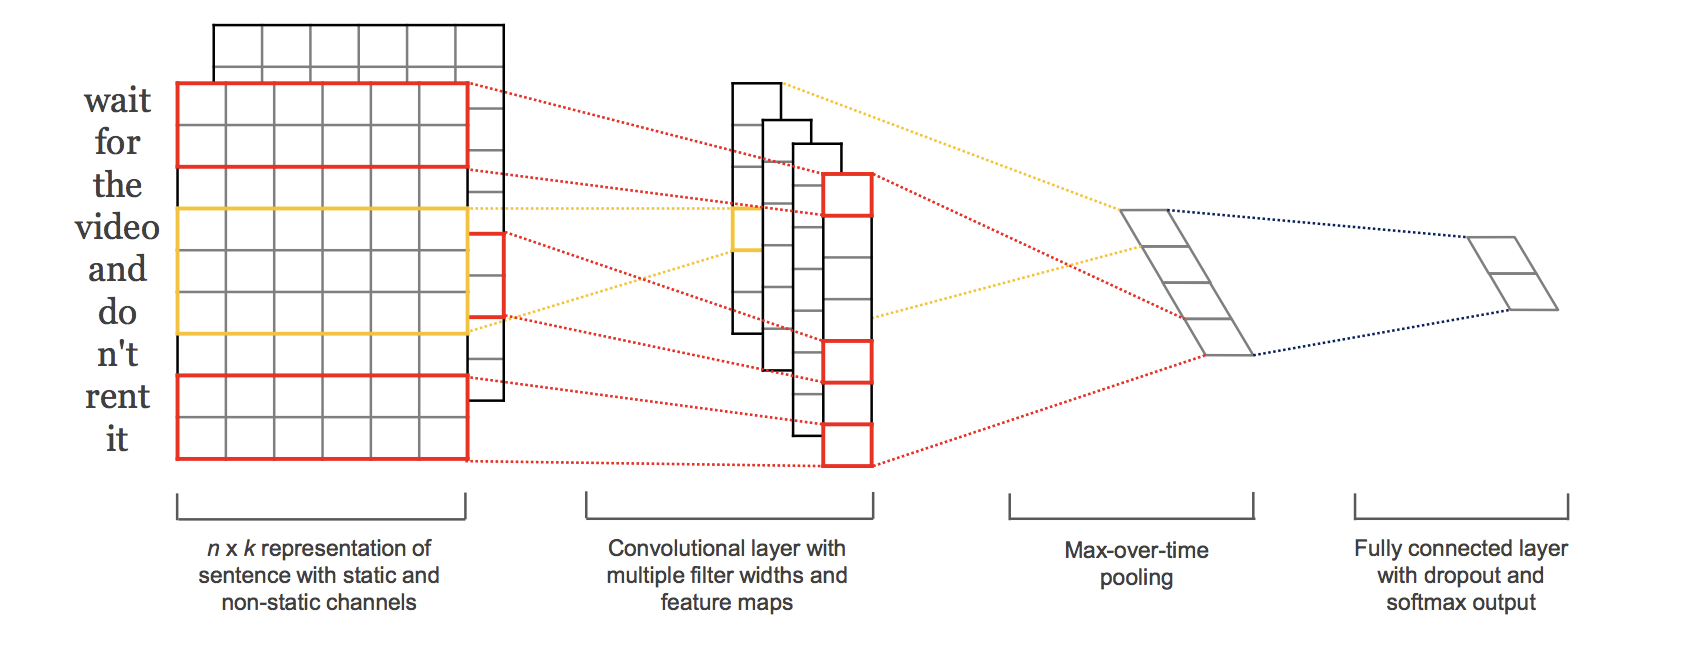
\includegraphics[scale=0.5]{CNN.png}
      \caption{An illustration of an n-gram convolutional neural network. The input is a numerical representation (\ref{section:embeddings}) of a tokenized text. The convolution over the input matrix is represented as a red and yellow box (called feature map) that is then pooled (maximum of the kernel). The classification is then enforced by a fully connected layer that incorporates the input of all feature maps.}
      \label{fig:cnn}
  \end{figure}

\subsection{Embeddings}\label{section:embeddings}
  In \ref{section:bow}, I introduced the bag-of-words approach to cope with the difficulty to explicitly model language, and in \ref{section:nbc} I showed that this approach even facilitates a good performing classifier.
  However, the bag-of-words approach models language incorrectly and having a better representation of language is more desirable for the improvement of ML algorithms.
  \textbf{Word embeddings}\index{word embeddings} are such methods that model language more accurately by representing words as n-dimensional vectors that much better capture syntactic and semantic characteristics of language.

\subsubsection{Word2Vec}\label{c:word2vec}
  In 2013, \citeauthor{Mikolov2013} published two algorithms to compute high quality distributed representations of words and phrases efficiently.
  Both these algorithms are also referred to as \textbf{word2vec}\index{word2vec}.
  The general approach in both algorithms is to maximize the similarity measures of vectorized words that appear in a similar context.
  The \textbf{continuous bag-of-words model}\index{continues bag-of-words model} is trained to predict the vector representation of a word or phrase given $n$ words before and after the target word in its sentence.
  The \textbf{continuous skip-gram-model}\index{continuous skip-gram-model} is a slower implementation with the benefit to model uncommon words better \citep{word2vec}.
  The skip-gram-model tries to predict the context given a target word and is thus the opposite approach of the continuous bag-of-words model.

  In practice, we generate labeled data in the form of tuples $(\mathbf{w}_t, \mathbf{w}_{c_{1}}, \dots, \mathbf{w}_{c_{n}})$, where one entry is the target word $\mathbf{w}_t$, and the other entries are context words $\mathbf{w}_c$.
  The tuple can either contain actual context words found in the text, or random words from the vocabulary (\textbf{negative sampling}\index{negative sampling}).
  The embedding layer learns the weights of the input and context words, by yielding an n-dimensional vector for all these words, calculates the dot-product of the target and context vectors in the merge-layer, and then passes it to a sigmoid layer that predicts whether the words are actual context words or were negatively sampled.
  The objective of the algorithm is to maximize
  \[\sum_{t \in T} \sum_{c \in \mathcal{C}_t} log( p(\mathbf{W}_c|\mathbf{w}_t))\]
  where $\mathbf{w}$ is the vector representation of a word, $t$ is the target word and $\mathbf{W}_c$ the context matrix, where each row is a vector representation of a context word.

\subsubsection{GloVe}\label{c:glove}
  Word2vec embeddings are local since only $n$ surrounding words are considered to calculate the embedding.
  \textbf{GloVe}\index{GloVe}, on the other hand, also tries to incorporate global information about word occurrences.

  As the first step, a word co-occurrence matrix over all documents is calculated.
  The underlying assumption of GloVe is that the co-occurrence ratio is connected to meaning.
  Let $X_{ij}$ be the co-occurrence count of token $j$ in the context of $i$. Let $X_i = \sum_{t \in T} X_{it}$ be the occurrence of token i given any other token then $p(j|i) = \frac{X_{ij}}{X_i}$ is the probability of token $j$ appearing in the context of token $i$.
  To be able to model the semantic information of words, their relationship needs to be modeled.
  GloVe defines a function $F((\mathbf{w_i} - \mathbf{w_j})^T \widetilde{w_t}) = \frac{p(i|k)}{p(j|k)}$ where $\mathbf{w}$ is a real-valued word vector.
  Hereby, the context words are subtracted from the input words, and the dot product with the weights of the output vocabulary is taken (see \cite{Pennington2014} for details).
  This step facilitates embedding arithmetic, i.e., the meaning of word embeddings can be deducted from arithmetic calculations such as $w_{man} + w_{royalty} = w_{king}$.
  Further steps are required for computability, such as weighting of the word vectors or handling zero entries which are described by \cite{Pennington2014}.

%\subsubsection{BERT}
\subsubsection{Document Embedding}
  If an algorithm only needs to operate on the document level, then the whole document can be embedded.
  A simple approach is to take the mean or the maximum of all word embeddings of a document.
  There are also more elaborated methods \citep{Wu2018, Liu2018, Andrew2015} that have a learning objective, similar to word embeddings.
  However, their downside is the demand for a large corpus to learn a meaningful \textbf{document embedding}\index{document embedding} which is not available in the scope of this thesis.

% \subsection{Web Scraping}
%   The process of automatically extracting content available on the world wide web is called \textbf{web scraping}\index{web scraping}.
%   It is different from web crawling, where the primary purpose is the following of hyperlinks on websites to index the linkage between pages.
%   However, both techniques can be combined to systematically search for some specific content within a network of websites, e.g., crawling flight provider sites and monitor their prices.

% \subsubsection{HTML and CSS}
%   \textbf{Hypertext Markup Language} (\GLS{HTML})\index{HTML} is a markup language which means that it consists of a set of \textsl{tags} that define how the content of a document needs to be interpreted.
%   In HTML, for example, \mintinline{HTML}{<h1> I am a Header </h1>} defines the opening of a header tag followed by some content and the closing of this tag.
%   When this HTML code is interpreted, the text is then displayed bold and larger than non-header text if not specified otherwise.

%   \textbf{Cascading Style Sheets} (\GLS{CSS})\index{CSS} is a style sheet language that is used for styling HTML code.
%   Given the example above, we could modify the header to have another color, \mintinline{HTML}{<h1 style="color:red">  I am a Header </h1>}.
%   It is also possible to define a \textbf{CSS class} and use this class to automatically apply several styles such as in Lis. \ref{lst:css},
%   %
%   \begin{listing}[h!]
%     \centering
%     \begin{cminted}{CSS}
%       .header {
%         color: red;
%         font-family: verdana;
%       }
%     \end{cminted}
%     \caption{CSS class named \emph{header} that sets the font to verdana and color to red when used.}
%     \label{lst:css}
%   \end{listing}
%   %
%   This way, we can apply the style like so \mintinline{HTML}{<h1 class="header"> I am a Header </h1>}.
%   While a class can be accessed from several HTML tags, there is also a \textbf{CSS id} that can only be accessed once in one HTML file but otherwise has the same functionality as a CSS class.
%   Both languages thereby reveal a way of filtering the content of a website.
%   Web scraping is exploiting HTML tags and CSS selectors like classes or ids to filter the content of a site.

%   Important tags for scraping are the paragraph tag \mintinline{HTML}{<p>} that normally contains text intended for the reader of a website and the \mintinline{HTML}{<a>} tag that contains hyperlinks.
%   By investigating websites thoroughly, one might also find a schema in the assignment of CSS selectors that can be exploited during web scraping.

  \[\dots\]
% \subsubsection{REST}
%   Most websites offer a web service which is a broad term for some user interface that allows the communication to a database and optionally performs some operation on this data.
%   The usual implementation of an application program interface is the \textbf{Representational State Transfer} (\GLS{REST}), and its methods are GET, POST, PUT, PATCH, and DELETE which are often executed via HTTP.
%   The most important method in web scraping is the GET method since it retrieves data.
%   It is sometimes necessary to understand how GET requests are made on a website to use them for automated content extraction.

% \subsubsection{Ajax}
%   Should the client (user) request data from a database via a website and a reload of the site is undesired, \textbf{Ajax}\index{Ajax} allows an asynchronous data retrieval.
%   This asynchronous GET request starts on an event (e.g., clicking on a button on the website).
%   Ajax is frequently used to reduce loading time and traffic to only refresh the necessary part of a website.
%   One framework to use Ajax is \textbf{jQuery} which is mostly used in combination with JavaScript that is required to integrate the retrieved data into the website.

%   A problem of scraping and crawling programs is that content, which is only visible after Ajax has requested it, is not visible to the program.
%   Therefore, it might be necessary to monitor the website's behavior via the developer mode of a web browser and see which GET requests would retrieve the data of interest or trigger the Ajax calls programmatically.
